% !TEX root = ../main.tex
%%--------------------------------------------------------------------------
%% SCENARIOS
%%--------------------------------------------------------------------------



\chapter{Data Design}

This chapter describes the stages of the design of the database. Specifically, it addresses the conceptual design, which models the reality of the system by identifying the main entities and their relationships; the conversion of these entities and their relationships in their implementation will be an adaptation to the non-relational database of Google App Engine.
The entities involved are a few: User, Pomotask and Pomodoro.

		\begin{figure}[h!]
		  \centering
		    \centering{%
		      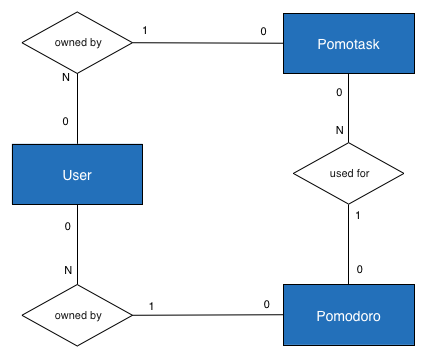
\includegraphics[width=1\textwidth]{er.png}}
		  \caption{Entity Diagram}
		\end{figure}
